\section{Advanced Hardware Construction in Chisel}
Another way to support hardware facilities in Chisel, as opposed to
building new nodes, is to write a Scala program that aggregates the
features of Chisel from Chapter~\ref{sec:chisel} into a directed graph
of nodes that implement the same hardware functionality. This approach
has the advantage of decoupling the hardware facility from the
backend, making the hardware facility more accessible as it can now be
mapped to more backends. The only requirement on the backend is that
they can support the basic Chisel nodes from
Chapter~\ref{sec:chisel}. Furthermore, the designer is no longer
required to write the code generation function for every single
backend, saving a great deal on designer effort. The rest of this
chapter will show how to implement ListLookup and Vec using only the
basic Chisel nodes presented in Chapter~\ref{sec:chisel}

\subsection{ListLookup}
\begin{figure}[htb]
\centering
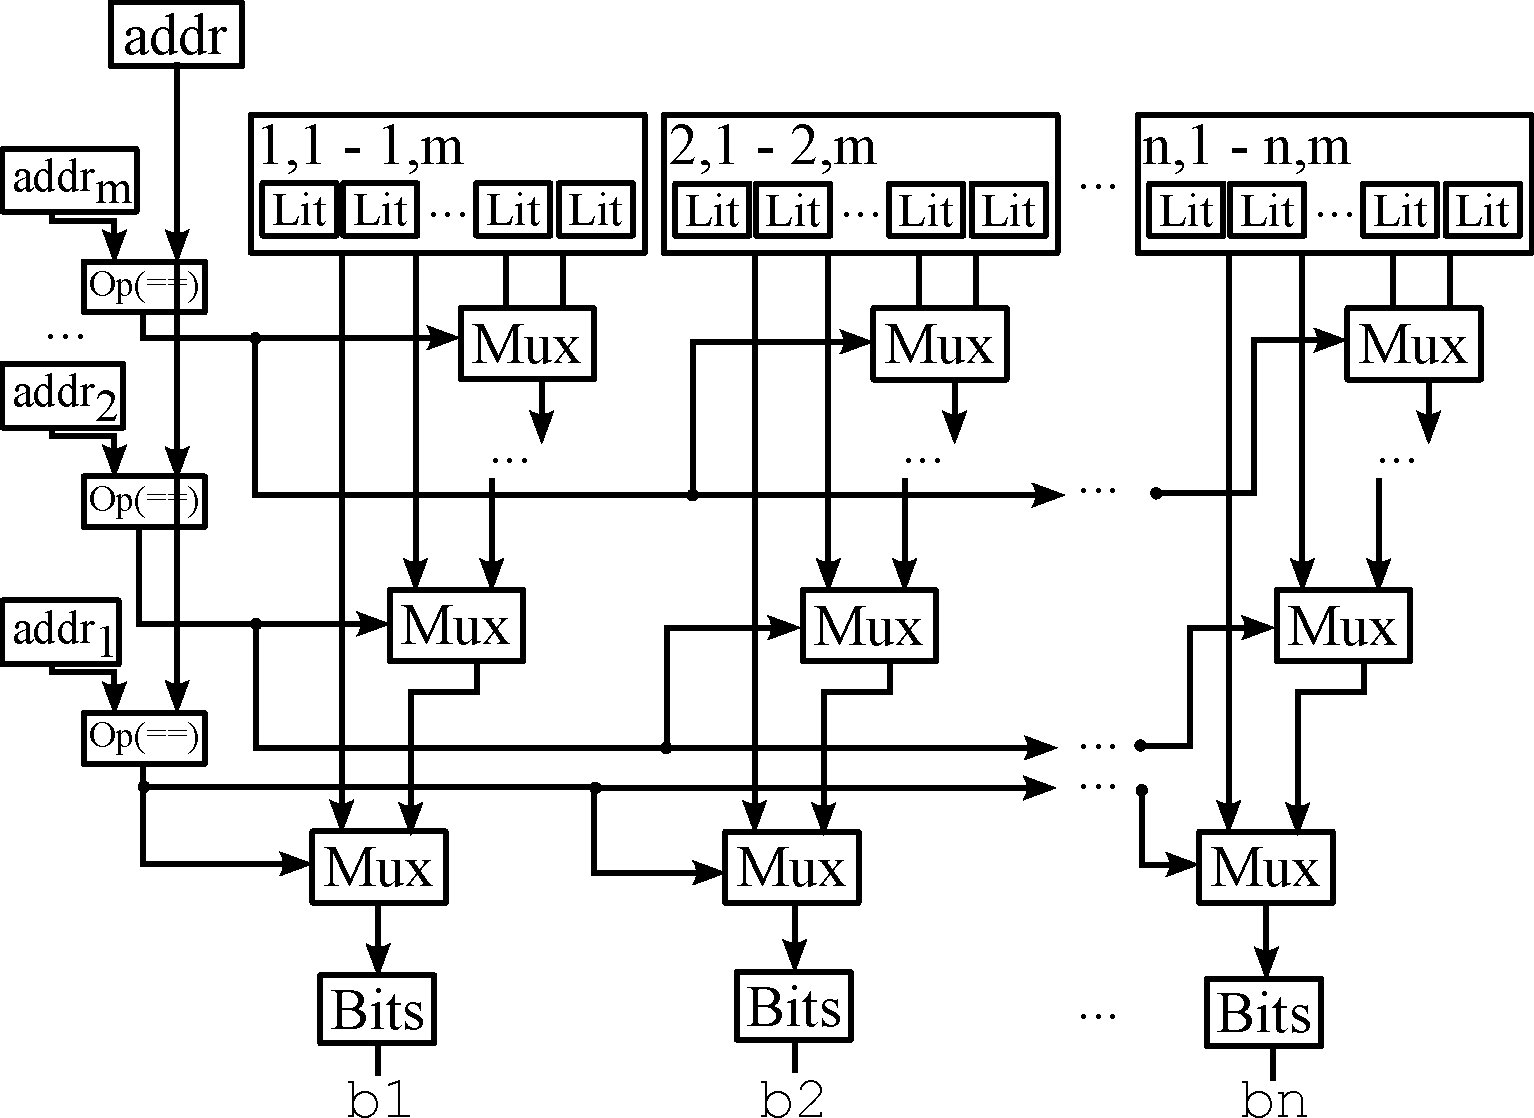
\includegraphics[width=0.7\textwidth]{figures/listlookupscala.pdf}
\caption{ListLookup implemented using Scala code and basic Chisel nodes}
\label{fig:llscala}
\end{figure}

The syntax for ListLookup remains the same. Users provide an address
for lookup and a list of size $m$ of tuples {\tt ($a_i$, $lits_i$)}
where {\tt $a_i$} is the address to match the lookup address against and
{\tt $lits_i$} is a list of size $n$ of literals to return when there
is a match. The ListLookup will then construct the graph in
Figure~\ref{fig:llscala}. The function returns a list of {\tt Bits}
{\tt $b_1$, ... $b_n$} who will take on the values of {\tt $lits_i$} if
{\tt $a_i$} matches the lookup address.

ListLookup graphs are constructed as follows. Given the input list of
tuples {\tt ($a_i$, $lits_i$)}, create $n$ list of $m$ tuples
{\tt $( (a_1, l_{1, k}), ... (a_j, l_{j, k}), ..., (a_m, l_{m, k})
  )$}. Each of these list represents a mux chain and there are $n$
such list ($k$ ranges from 1 to $n$). The mux chains are constructed
using {\tt $a_i$ === addr} as the select signal to the corresponding
mux. If the address matches, then literal {\tt $l_{i, k}$} is ouputted
for Bits $b_k$.

\subsection{Vec}
\begin{figure}[htb]
\centering
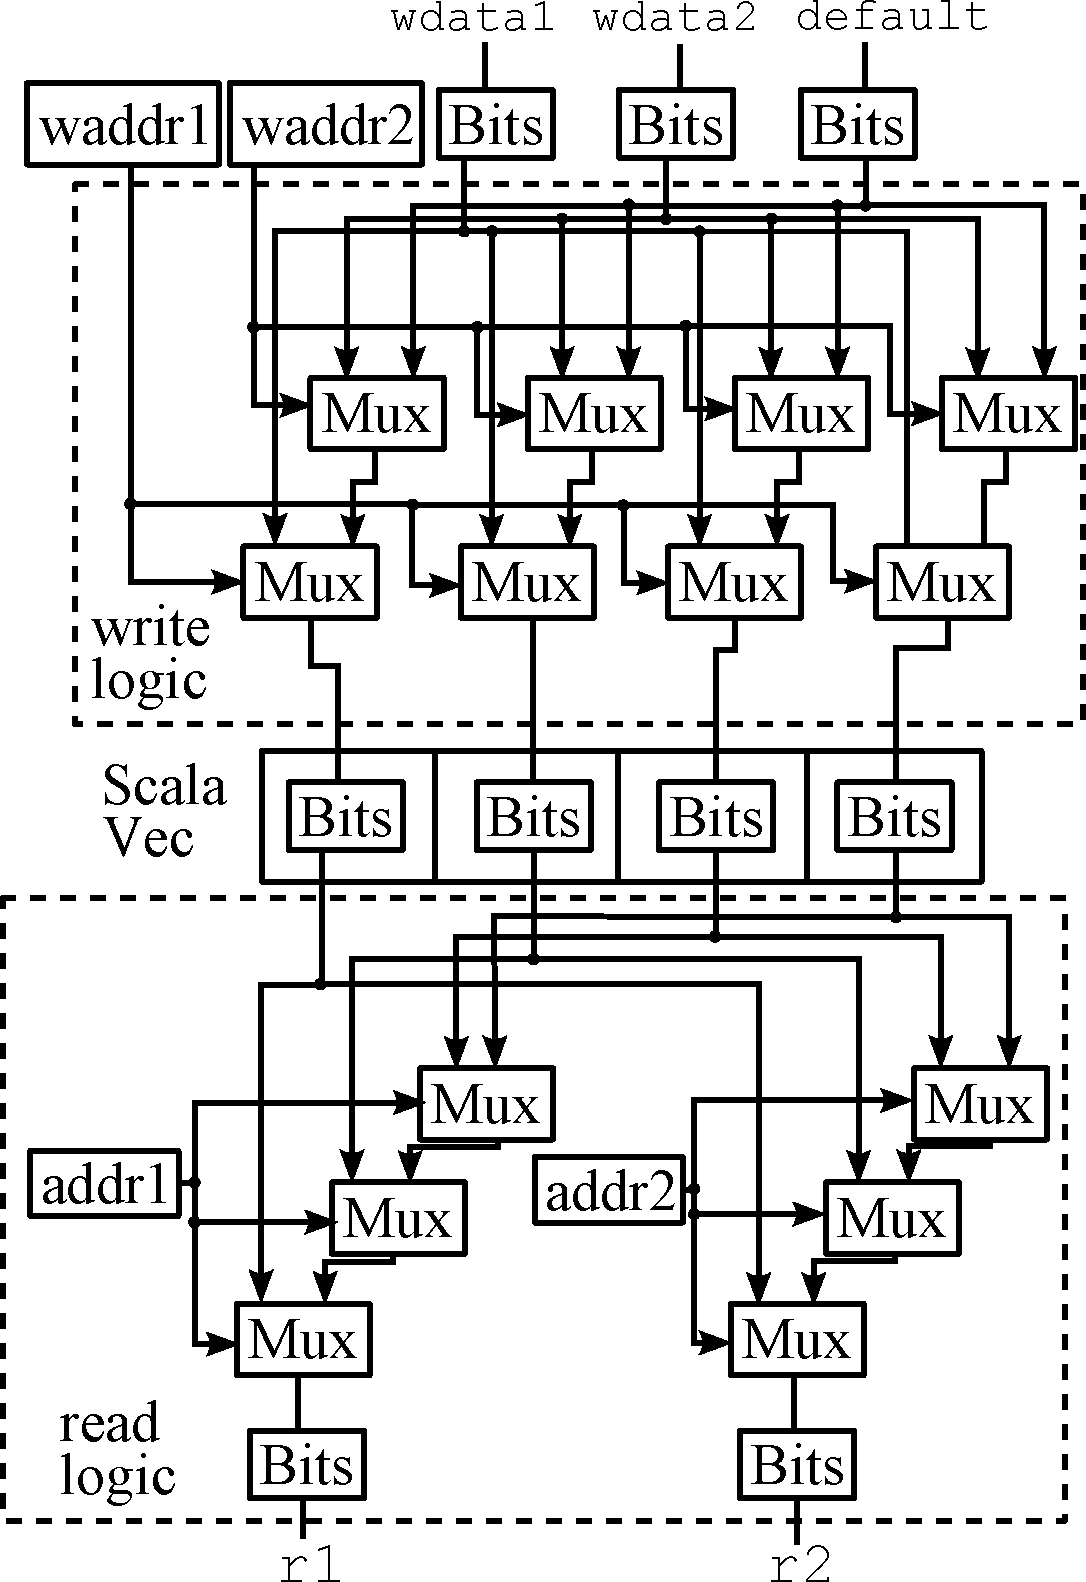
\includegraphics[width=0.5\textwidth]{figures/vecscala.pdf}
\caption{Vec implemented using Scala code and basic Chisel nodes}
\label{fig:vecscala}
\end{figure}
